\newpage
\section{Wichtigkeit der Features}
\label{sec:eval_feature_importance}
Die Wichtigkeit, oder Signifikanz, der Features wird in dieser Arbeit definiert als der Fehler,
der durch die Modifizierung eines Features in der Testmenge im Vergleich zur ursprünglichen Testmenge entsteht.
Die Permutationswichtigkeit ist der Fehler, der durch das permutieren eines Features in der Testmenge entsteht, im Vergleich zu der ursprünglichen Testmenge.
Je größer der Fehler, desto wichtiger das Feature \cite{breiman2001random}.
\newline
\newline
Scikit-Learn bietet für den verwendeten \textit{RandomForest} ein Attribut \texttt{feature\_importances\_} an, dass die Feature-Wichtigkeit ausgeben soll.
Dieses beschreibt die akkumulierte \textit{Impurity}-Verringerung, das ein Feature im Entscheidungswald beiträgt \cite{ScikitLearnFeatureImportance}.
Dabei gibt \textit{Purity} an, wie durchmischt die Klassen in den Blättern der Entscheidungsbäume sind,
d.~h. Features die früh in der Konstruktion verwendet werden, haben laut dieser Metrik einen großen Einfluss.
Zur besseren Vergleichbarkeit mit den FFNNs wurde diese Metrik aber nicht verwendet.
\newline
\newline
Abbildung \ref{fig:fi_consolidated} zeigt die Permutationswichtigkeiten der ML-Modelle mit Rückwärtskante zur Standortbestimmung.
Die Features sind abgekürzt in der Grafik: \textit{acc} steht für die Features aus den Accelerometer, \textit{light} für den Lichtsensor, \textit{ap} für den WLAN-Zugangspunkt,
\textit{temperature} für den Temperatursensor, \textit{heading} für den Magnetfeldsensor, \textit{volume} für den Geräuschsensor, \textit{ang} für das Gyroskop.
\newpage
Auffallend ist, dass die Features der vorherigen Standorte keine Wichtigkeit haben.
Dies ist durch das iterative Evaluierungsverfahren der Testmenge begründet,
d.~h. eine Permutation hat keinen Effekt, da diese Features während der Evaluierung von dem Modell selbstständig bestimmt werden.
\begin{figure}[h!]
    \centering
    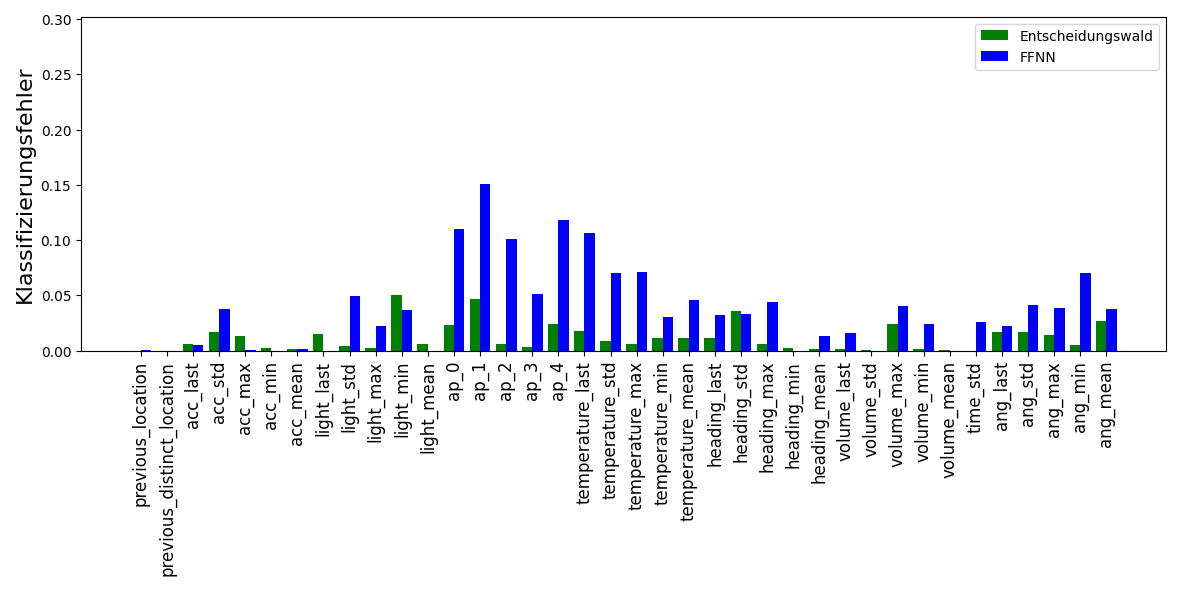
\includegraphics[width=\linewidth]{images/fi_consolidated.png}
    \caption{Permutationswichtigkeit der Features der ML-Modelle mit Rückwärtskante.}
    \label{fig:fi_consolidated}
\end{figure}
\newline
Insgesamt ist der Entscheidungswald sehr robust gegenüber der Permutation eines einzelnen Features.
Der größte Fehler wird durch die Permutation des Minimums der Lichtintensität induziert.
Das FFNN hingegen ist deutlich anfälliger gegenüber der Permutation eines einzelnen Features.
Der größte Fehler ist 15,1 Prozentpunkte gegenüber 5,0 Prozentpunkte des Entscheidungswaldes.
\newline
\newline
Die wichtigsten Features für den Entscheidungswald sind das Minimum der Lichtintensität, die WLAN-Zugangspunkte, die Standardabweichung zu der Ausrichtung zum Magnetfeld,
das Maximum der Lautstärke und der Durchschnitt der Drehbeschleunigung.
Damit nutzt der Entscheidungswald mindestens ein Feature aus jeder Feature-Art.
Je nach Sensortyp sind einige Feature-Arten nicht so aussagekräftig, wie andere Feature-Arten.
\newline
\newline
Auffallend ist, dass dort wo der Durchschnitt nicht aussagekräftig ist, das Minimum oder das Maximum stattdessen Aussagekraft besitzt.
Insbesondere trifft dies auf die Beschleunigung des Accelerometers, der Lichtintensität und der Lautstärke zu.
Diese haben gemeinsam, dass der Großteil ihrer Sensorwerte sehr ähnlich sind,
d.~h. eine gleichbleibende Beschleunigung, Lichtintensität oder Lautstärke.
Extrema weisen auf besondere Standorte hin, bei denen sich die Sensorwerte ruckartig ändern.
Damit diese in der Permutationswichtigkeit relevant sind, müssen diese relativ häufig vorkommen.
\newpage
Unerwartet ist, dass das Minimum der Lichtintensität, im Gegensatz zum Maximum, eine hohe Aussagekraft besitzt, da die platzierten Lichtquellen die Lichtintensität nur erhöhen.
Vermutlich wird das Minimum verwendet, um sich von den üblichen Lichtintensitäten zu unterscheiden, anstatt mit dem Maximum nach speziellen Standorten zu suchen.
\newline
\newline
Bei den Features zu der Ausrichtung zum Magnetfeld und der Beschleunigung wird zudem die Standardabweichung benutzt.
Diese drückt signifikante Änderungen im Datenfenster aus.
Besonders bei der Ausrichtung zum Magnetfeld ist eine Unterscheidung basierend auf Extrema nicht sinnvoll,
da die Ausrichtung zum Magnetfeld abhängig von der Orientierung der Sensorenbox ist, die sich im Laufe der Route ändern kann.
\newline
\newline
Besonders relevant sind zudem die Detektierung der WLAN-Zugangspunkte und alle Features basierend auf den Sensorwerten des Gyroskops.
Die WLAN-Zugangspunkte sind binär.
Eine Detektierung schließt bestimmte Standorte direkt aus, weswegen die Wichtigkeit nachvollziehbar ist.
In der Simulation dreht sich die Sensorenbox an vielen Ecken, weswegen die Sensorwerte für diese Standorte sehr Aussagekräftig sind.
Eine durchschnittliche Drehbeschleunigung weißt auf diese Standorte konsistent hin.
\newline
\newline
Das FFNN weißt den gleichen Features ebenfalls eine hohe Wichtigkeit zu, nur ist der verursachte Fehler durch die Permutation bis zu drei-mal größer.
Im Gegensatz zum Entscheidungswald, ist die Wichtigkeit der Standardabweichung und des Maximums der Lichtintensität größer und das Minimum dafür geringer.
Dies ist nachvollziehbar, wenn man betrachtet, dass bei Standorten in der Umgebung von Lichtquellen die Lichtintensität kontinuierlich steigt.
Zudem ist die Wichtigkeit der Features des Temperatursensors deutlich höher.
Die Temperatur verhält sich ähnlich zur Lichtintensität.
In der Nähe von Wärmequellen verändert sich die Temperatur kontinuierlich, bis ein Maximum oder Minimum erreicht wird.
Unerwartet ist die Wichtigkeit, die dem Maximum der Ausrichtung zum Magnetfeld zugewiesen wird.
Wie zuvor diskutiert, ist dieses Feature fachlich nicht sinnvoll.
\newline
\newline
Abbildung \ref{fig:fi_consolidated_wo_fb} zeigt die Permutationswichtigkeit der ML-Modelle ohne Rückwärtskante zur Standortbestimmung.
Die Wichtigkeit der Features für den Entscheidungswald sind weitestgehend unverändert,
wobei die verursachten Fehler durch die Permutation größer sind, im Vergleich zum Entscheidungswald mit Rückwärtskante.
Ähnlich verhält sich auch das FFNN im Vergleich zum FFNN mit Rückwärtskante.
Die Wichtigkeit der Standardabweichung, sowie der Wert der Temperatur ist geringer.
\begin{figure}[h!]
    \centering
    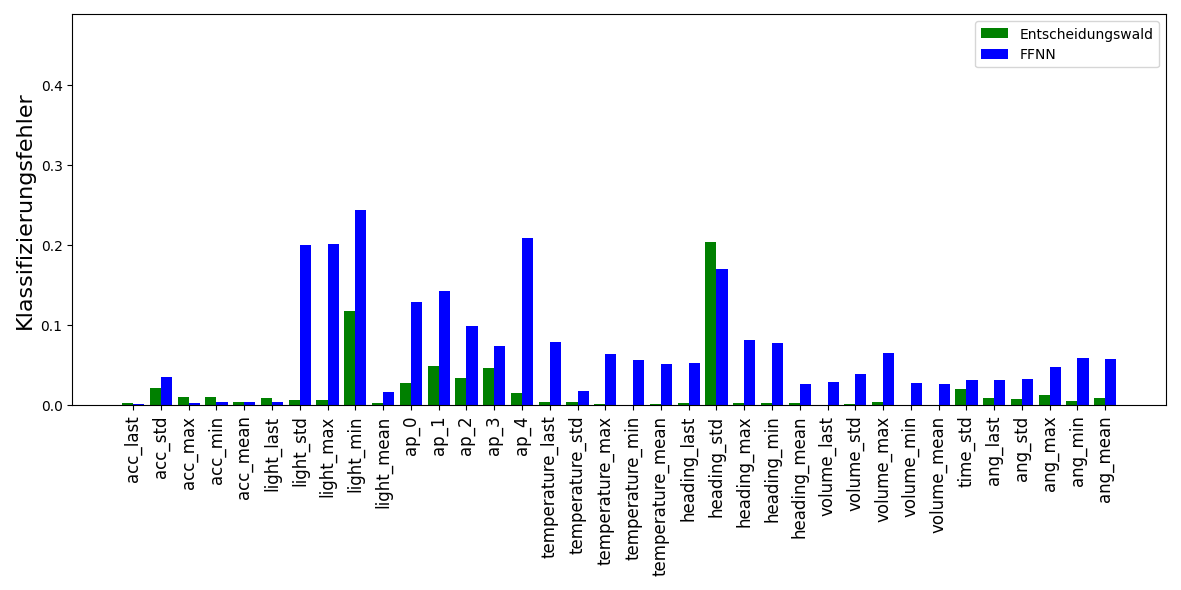
\includegraphics[width=\linewidth]{images/fi_consolidated_wo_fb.png}
    \caption{Permutationswichtigkeit der Features der ML-Modelle ohne Rückwärtskante.}
    \label{fig:fi_consolidated_wo_fb}
\end{figure}
\newpage
Abbildung \ref{fig:feature_significance_dt_anomaly} zeigt die Permutationswichtigkeit von einem Entscheidungswald zur Anomalieerkennung.
Am wichtigsten sind die Features, welche die Wahrscheinlichkeitsverteilung des Klassifizierungsergebnisses von dem ML-Modell zur Standortbestimmung ausnutzen.
Die Abweichung zu den durchschnittlichen Standortänderungen hat kaum Einfluss.
Dies deutet darauf hin, dass die ML-Modelle zur Standortbestimmung nicht so instabil in Anomalien sind.
Aus dem selben Grund hat das Feature der Topologieverletzung auch wenig Einfluss, da es bei Anomalien wenig ausschlägt.
Dem FFNN wird für jedem Feature die gleiche Wichtigkeit zugewiesen (Abbildung \ref{fig:fi_knn_anomaly}).
\begin{figure}[h!]
    \centering
    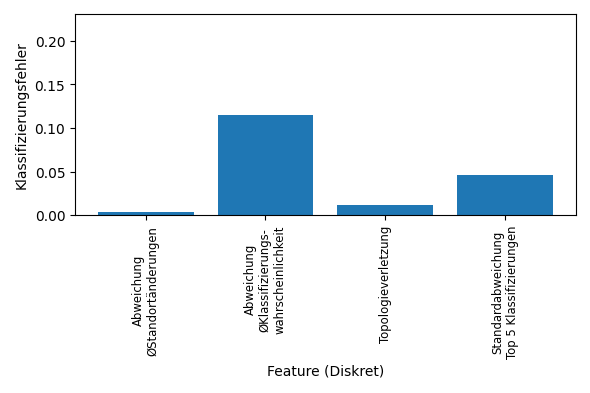
\includegraphics[width=0.65\linewidth]{images/fi_anomaly_dt.png}
    \caption{Permutationswichtigkeit der Features eines Entscheidungswaldes zur Anomalieerkennung.}
    \label{fig:feature_significance_dt_anomaly}
\end{figure}
\newline
\newline
Die Wichtigkeit der Features variiert mit dem Szenario, indem die ML-Modelle eingesetzt werden, und unter den einzelnen ML-Modellen.
Aus diesem Grund sollte die Analyse der Wichtigkeit der Features individuell für jedes Einsatzszenario und ML-Modell durchgeführt werden,
womit durch eine sorgfältige Feature-Selektion die Klassifizierungsgenauigkeit maximiert und der Ressourcenverbrauch minimiert werden kann.